\section*{Approach}
%\FloatBarrier

The system consists of two separate parts; an unsupervised algorithm for
augmenting data, and a supervised algorithm for classifying the data (Figure
\ref{fig:overview}). The unsupervised portion attempts to augment the data with
additional structural information. It could be considered a preprocessing step,
with the choice of parameters acting as a way to inject some amount of domain
knowledge into the data. The supervised portion consists of a regular
classification algorithm.

\begin{figure}[htbp]
  \centering
  \missingfigure[figwidth=\textwidth]{Layout of the system}
  \caption{A high-level overview of the system}
  \label{fig:overview}
\end{figure}

\subsection*{Unsupervised}
The unsupervised algorithm attempts to detect and label blocks of text in the
PDF file, as shown in Figure \ref{fig:clustered} for an example). This approach
is based on work by \textcite{klampfl2014unsupervised}, and consists of two
clustering steps:
\begin{enumerate}
\item Individual letters are clustered together into blocks of semantically
  relevant text (e.g. a full paragraph, or a section header).
\item These blocks are labeled by a different clustering algorithm.
\end{enumerate}

\begin{figure}[htb]
  \centering
  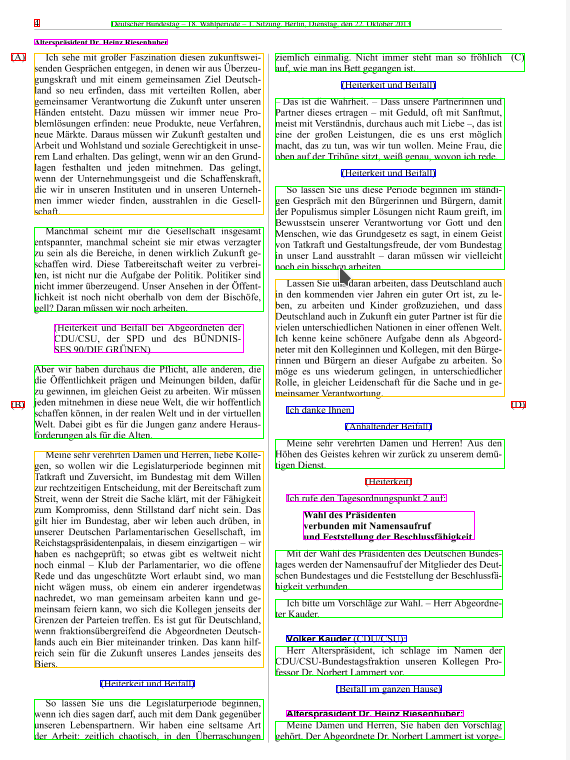
\includegraphics[height=0.5\textheight]{figures/cluster_example.png}
  \caption{An example of clustered blocks of text, blocks with the same outline
    color belonging to the same cluster.}
  \label{fig:clustered}
\end{figure}

\subsubsection*{Hierarchical Agglomerative Clustering}
The first step is performed using hierarchical agglomerative clustering (HAC),
an unsupervised bottom-up clustering algorithm that constructs a hierarchical
tree of clusters (in this context referred to as a \emph{dendrogram}). An
example is shown in Figure \ref{fig:hac}. The algorithm gets fed the individual
characters present in the PDF files, then iteratively groups the two closests
clusters (the initial inputs being regarded as clusters of one element) together
until only a single cluster remains. This process involves two parameters:
\begin{enumerate}
\item The distance function between two characters.
\item The distance function between two groups of characters.
\end{enumerate}
The first parameter is trivially chosen to be the Euclidian distance between the
coordinates of the two characters. The second parameter is called the
\emph{linkage} and has several common options, the most basic of which are:
\begin{itemize}
\item Single-linkage: The distance between groups is based on the closest two
  elements: \[ d(A, B) = \min \{ d(a, b) : a \in A, b \in B \} \]
\item Maximum-linkage: The distance between groups is based on the furthest two
  elements: \[ d(A, B) = \max \{ d(a, b) : a \in A, b \in B \} \]
\item Average-linkage: The distance between groups is based on the furthest two
  elements: \[ d(A, B) = \frac{1}{|A||B|} \sum_{a \in A}\sum_{b \in B} d(a, b) \]
\end{itemize}
As per \textcite{klampfl2014unsupervised}, single-linkage clustering performs
best for this task due to its tendency to form long thin clusters, mimicking the
structure of sentences. As an additional bonus, while the general time
complexity for HAC is in $\mathcal{O}(n^3)$, single-linkage clustering can be
done in $\mathcal{O}(n^2)$ \citep{sibson1973slink}, making it far more usable on
medium-sized datasets.

\begin{figure}[htb]
  \centering
  \begin{subfigure}[b]{0.49\textwidth} 
    \centering
    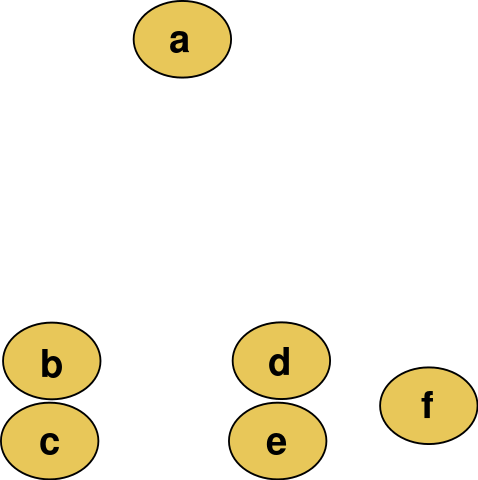
\includegraphics[width=\textwidth]{figures/dendrogram1.png}
    \caption{Before}
  \end{subfigure}
  \begin{subfigure}[b]{0.49\textwidth}
	\centering
    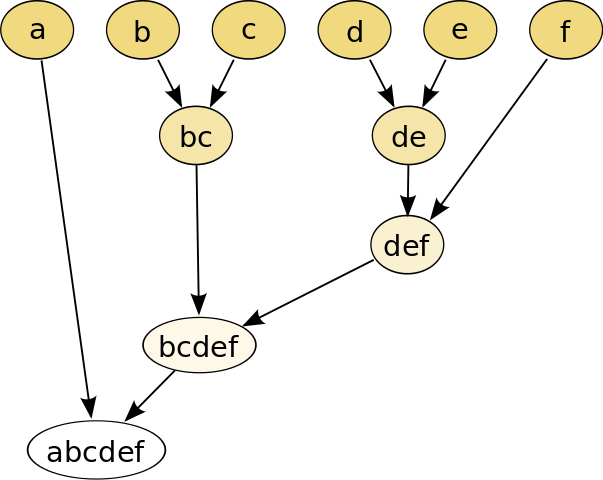
\includegraphics[width=\textwidth]{figures/dendrogram2.png}
    \caption{After}
  \end{subfigure}
  \caption{An example of hierarical agglomerative clustering.}
  \label{fig:hac}
\end{figure}

After the dendrogram is concstructed, the only choice left is at which level to
cut the tree to obtain the desired blocks of text. This is left as a parameter
to be manually finetuned.

\subsubsection*{Classical Clustering}
The extracted blocks from the previous step are then clustered according to
the similarity of their shapes (width and height). This is done using K-means
clustering for some chosen $K$, or with the DBSCAN algorithm.
\todo{Either expand this section or integrate it with the previous subsubsection
and just remove the subsubsection header.}
\subsection*{Supervised}
